\documentclass[11pt]{article}

\usepackage{times}
\usepackage{epsf}
\usepackage{epsfig}
\usepackage{amsmath, alltt, amssymb, xspace}
\usepackage{wrapfig}
\usepackage{fancyhdr}
\usepackage{url}
\usepackage{verbatim}
\usepackage{fancyvrb}

\usepackage{subfigure}
\usepackage{cite}
%\usepackage{cases}
%\usepackage{ltexpprt}
%\usepackage{verbatim}

%\topmargin      -0.70in  % distance to headers
%\headheight     0.2in   % height of header box
%\headsep        0.4in   % distance to top line
%\footskip       0.3in   % distance from bottom line

% Horizontal alignment
\topmargin      -0.50in  % distance to headers
\oddsidemargin  0.0in
\evensidemargin 0.0in
\textwidth      6.5in
\textheight     8.9in 


%\centerfigcaptionstrue

%\def\baselinestretch{0.95}


\newcommand\discuss[1]{\{\textbf{Discuss:} \textit{#1}\}}
%\newcommand\todo[1]{\vspace{0.1in}\{\textbf{Todo:} \textit{#1}\}\vspace{0.1in}}
\newtheorem{problem}{Problem}[section]
%\newtheorem{theorem}{Theorem}
%\newtheorem{fact}{Fact}
\newtheorem{define}{Definition}[section]
%\newtheorem{analysis}{Analysis}
\newcommand\vspacenoindent{\vspace{0.1in} \noindent}

%\newenvironment{proof}{\noindent {\bf Proof}.}{\hspace*{\fill}~\mbox{\rule[0pt]{1.3ex}{1.3ex}}}
%\newcommand\todo[1]{\vspace{0.1in}\{\textbf{Todo:} \textit{#1}\}\vspace{0.1in}}

%\newcommand\reducespace{\vspace{-0.1in}}
% reduce the space between lines
%\def\baselinestretch{0.95}

\newcommand{\fixmefn}[1]{ \footnote{\sf\ \ \fbox{FIXME} #1} }
\newcommand{\todo}[1]{
\vspace{0.1in}
\fbox{\parbox{6in}{TODO: #1}}
\vspace{0.1in}
}

\newcommand{\mybox}[1]{
\vspace{0.2in}
\noindent
\fbox{\parbox{6.5in}{#1}}
\vspace{0.1in}
}


\newcounter{question}
\setcounter{question}{1}

\newcommand{\myquestion} {{\vspace{0.1in} \noindent \bf Question \arabic{question}:} \addtocounter{question}{1} \,}

\newcommand{\myproblem} {{\noindent \bf Problem \arabic{question}:} \addtocounter{question}{1} \,}


\newcommand{\copyrightnoticeA}[1]{
\vspace{0.1in}
\fbox{\parbox{6in}{\small Copyright \copyright\ 2006 - 2014\ \ Wenliang Du, Syracuse University.\\ 
      The development of this document is partially funded by 
      the National Science Foundation's Course, Curriculum, and Laboratory 
      Improvement (CCLI) program under Award No. 0618680 and 0231122. 
      Permission is granted to copy, distribute and/or modify this document
      under the terms of the GNU Free Documentation License, Version 1.2
      or any later version published by the Free Software Foundation.
      A copy of the license can be found at http://www.gnu.org/licenses/fdl.html.}}
\vspace{0.1in}
}


\newcommand{\copyrightnotice}[1]{
\vspace{0.1in}
\fbox{\parbox{6in}{\small Copyright \copyright\ 2006 - 2014\ \ Wenliang Du, Syracuse University.\\
      The development of this document is/was funded by three grants from
      the US National Science Foundation: Awards No. 0231122 and 0618680 from
      TUES/CCLI and  Award No. 1017771 from Trustworthy Computing.
      This lab was imported into the Labtainer framework by the Naval Postgraduate 
      School, Center for Cybersecurity and Cyber Operations under National Science 
      Foundation Award No. 1438893.
      Permission is granted to copy, distribute and/or modify this document
      under the terms of the GNU Free Documentation License, Version 1.2
      or any later version published by the Free Software Foundation.
      A copy of the license can be found at http://www.gnu.org/licenses/fdl.html.}}
\vspace{0.1in}
}

\newcommand{\copyrightnoticeB}[1]{
\vspace{0.1in}
\fbox{\parbox{6in}{\small Copyright \copyright\ 2006 - 2014\ \ Wenliang Du, Syracuse University.\\
      The development of this document is/was funded by the following grants from
      the US National Science Foundation: No. 0231122, 0618680, and 1303306.
      Permission is granted to copy, distribute and/or modify this document
      under the terms of the GNU Free Documentation License, Version 1.2
      or any later version published by the Free Software Foundation.
      A copy of the license can be found at http://www.gnu.org/licenses/fdl.html.}}
\vspace{0.1in}
}


\newcommand{\nocopyrightnotice}[1]{
\vspace{0.1in}
\fbox{\parbox{6in}{\small  
      The development of this document is funded by 
      the National Science Foundation's Course, Curriculum, and Laboratory 
      Improvement (CCLI) program under Award No. 0618680 and 0231122. 
      Permission is granted to copy, distribute and/or modify this document.
      }}
\vspace{0.1in}
}

\newcommand{\idea}[1]{
\vspace{0.1in}
{\sf IDEA:\ \ \fbox{\parbox{5in}{#1}}}
\vspace{0.1in}
}

\newcommand{\questionblock}[1]{
\vspace{0.1in}
\fbox{\parbox{6in}{#1}}
\vspace{0.1in}
}


\newcommand{\minix}{{\tt Minix}\xspace}
\newcommand{\unix}{{\tt Unix}\xspace}
\newcommand{\linux}{{\tt Linux}\xspace}
\newcommand{\ubuntu}{{\tt Ubuntu}\xspace}
\newcommand{\selinux}{{\tt SELinux}\xspace}
\newcommand{\freebsd}{{\tt FreeBSD}\xspace}
\newcommand{\solaris}{{\tt Solaris}\xspace}
\newcommand{\windowsnt}{{\tt Windows NT}\xspace}
\newcommand{\setuid}{{\tt Set-UID}\xspace}
%\newcommand{\smx}{{\tt Smx}\xspace}
\newcommand{\smx}{{\tt Minix}\xspace}
\newcommand{\relay}{{\tt relay}\xspace}
\newcommand{\isys}{{\tt iSYS}\xspace}
\newcommand{\ilan}{{\tt iLAN}\xspace}
\newcommand{\iSYS}{{\tt iSYS}\xspace}
\newcommand{\iLAN}{{\tt iLAN}\xspace}
\newcommand{\iLANs}{{\tt iLAN}s\xspace}
\newcommand{\bochs}{{\tt Bochs}\xspace}

\newcommand\FF{{\mathcal{F}}}

\newcommand{\argmax}[1]{
\begin{minipage}[t]{1.25cm}\parskip-1ex\begin{center}
argmax
#1
\end{center}\end{minipage}
\;
}

\newcommand{\bm}{\boldmath}
\newcommand  {\bx}    {\mbox{\boldmath $x$}}
\newcommand  {\by}    {\mbox{\boldmath $y$}}
\newcommand  {\br}    {\mbox{\boldmath $r$}}


%\pagestyle{fancyplain}
%\lhead[\thepage]{\thesection}      % Note the different brackets!
%\rhead[\thesection]{SEED Laboratories}
%\lfoot[\fancyplain{}{}]{Syracuse University} 
%\cfoot[\fancyplain{}{}]{\thepage} 

\newcommand{\tstamp}{\today}   
%\lhead[\fancyplain{}{\thepage}]         {\fancyplain{}{\rightmark}}
%\chead[\fancyplain{}{}]                 {\fancyplain{}{}}
%\rhead[\fancyplain{}{\rightmark}]       {\fancyplain{}{\thepage}}
%\lfoot[\fancyplain{}{}]                 {\fancyplain{\tstamp}{\tstamp}}
%\cfoot[\fancyplain{\thepage}{}]         {\fancyplain{\thepage}{}}
%\rfoot[\fancyplain{\tstamp} {\tstamp}]  {\fancyplain{}{}}

\pagestyle{fancy}
%\lhead{\bfseries Computer Security Course Project}
\lhead{\bfseries SEED Labs}
\chead{}
\rhead{\small \thepage}
\lfoot{}
\cfoot{}
\rfoot{}

\usepackage{listings}
\usepackage{color}

\definecolor{dkgreen}{rgb}{0,0.6,0}
\definecolor{gray}{rgb}{0.5,0.5,0.5}
\definecolor{mauve}{rgb}{0.58,0,0.82}

\lstset{frame=tb,
  language=C,
  aboveskip=3mm,
  belowskip=3mm,
  showstringspaces=false,
  columns=flexible,
  basicstyle={\small\ttfamily},
  numbers=none,
  numberstyle=\tiny\color{gray},
  keywordstyle=\color{blue},
  commentstyle=\color{dkgreen},
  stringstyle=\color{mauve},
  breaklines=true,
  breakatwhitespace=true,
  tabsize=3
}



\begin{document}

\begin{center}
{\LARGE Routing: Open Shortest First Path}
\vspace{0.1in}\\
\end{center}


\section{Overview}
This exercise introduces the Open Shortest First Path (OSPF) routing protocol,
allowing students to configure OSPF-enabled routers and view their behavior.
The student will use OSPF to spoof routing tables, leading to malicious mis-routing
of traffic.

OSPF is an internal gateway protocol (IGP).   The {\tt bird-bgp} lab explored the
Border Gateway Protocol (BGP), which is an external gateway protocol (EGP) used within the
Internet backbone, e.g., between ISPs.
This lab uses routers running the Bird service, which is an open source Linux-based router
implementation.

\subsection{Background}
This exercise assumes the student has received instruction on functions
of network routers, and OSPF.  
It is also assumed that the student is familiar with basic Linux routing, e.g., as explored in the
routing-basics and routing-basics2 labs.
There are a number of web-based resources describing OSPF.  Note however that many focus on Cisco
command line syntax and semantics.  Look for tutorials that explain concepts and not just rote 
steps needed to pass a certification.

This lab exercise only touches on some of the most basic elements of OSPF.

\section{Lab Environment}
This lab runs in the Labtainer framework,
available at http://my.nps.edu/web/c3o/labtainers.
That site includes links to a pre-built virtual machine
that has Labtainers installed, however Labtainers can
be run on any Linux host that supports Docker containers.

From your labtainer-student directory start the lab using:
\begin{verbatim}
    labtainer bird-ospf
\end{verbatim}
A link to this lab manual will be displayed, along with a link to the Bird router 
user guide.

\section{Lab topology}
The lab presents a simplified topology that includes of routers implementing OSPF within an Autonomous System (AS).  

In Figure \ref{fig:topology}, all of the components except those labeled \textit {External} are within one AS.
The {\tt BR} router is the border router for the AS.  The {\tt BRX} router is the border router for the 
notional external system.  The external system includes a web server, labeled {\tt WX}.
In addition to three internal routers, the AS has one server and three workstations.

The routers exchange routing information and traffic over the point-to-point ethernet
links.  Each such link has a network tap that forwards copies of traffic to the {\tt netmon} component (not pictured), 
which collects network traffic in files within its {\tt /taps} directory.

This lab primarily names computers using IP addresses.  Use of DNS is deliberately avoided to keep the focus on routing.

\begin{figure}[H]
\begin{center}
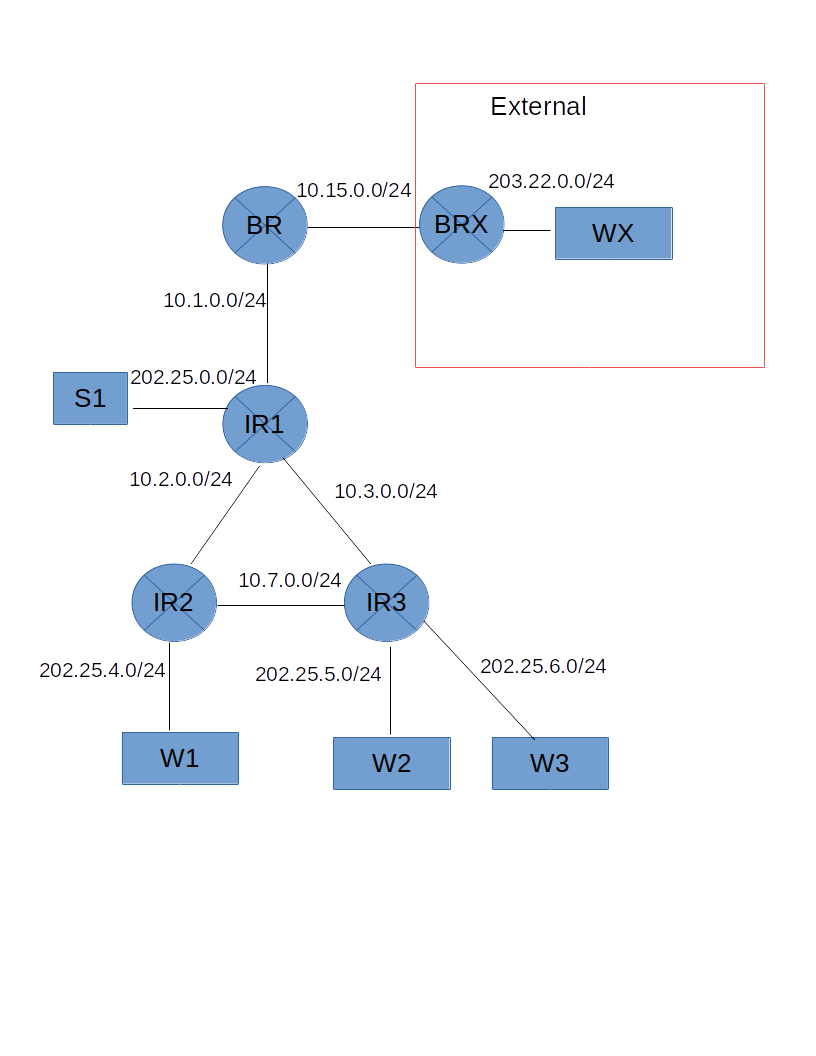
\includegraphics [width=0.8\linewidth]{topo.png}
\end{center}
\caption{OSPF Routing Topology}
\label{fig:topology}
\end{figure}

\section{Tasks}

\subsection{Explore}
The following items (among other), are available to explore the network:
\begin{itemize}
\item Wireshark and tcpdump are installed on the {\tt netmon} computer, use them to review the PCAP files found in
the {\tt /taps} directory.  When using Wireshark, if you encounter black or otherwise corrupt pulldown windows, try resizing the window,
or restarting the application.  The {\tt ctrl-r} key sequence will cause Wireshark to reload the PCAP file that is
currently being viewed, i.e., to see the latest traffic.
\item The {\tt traceroute} program is install on each computer (all components other than routers).  
Use that to observe the routes that traffic may take between different computers.
\item Each router includes the Bird client, which you can start using {\tt sudo birdc}.  Use it to view routes and
protocol definitions.  Bird is configured via use of configuration files found at {\tt /usr/local/etc/bird.conf}. 
The bird service runs under systemd.  If you modify a configuration file, you may rstart bird using {\tt systemctl restart
bird}.  The remaining tasks of this lab assume the bird.conf files on each router have not been modified.  If you do modify
those, either restore them, or restart that lab (using the {\tt -r} option on the {\tt labtainer} command prior to proceeding
to next steps.

\end{itemize}

\subsection{Confirm connectivity}
Use the {\tt ifconfig} command (or {\tt ip addr}) to determine IP addresses of the different computers.  
You should be able to ping any computer from any other.  You should also be able to use {\tt wget} to retrieve the index.html
file from the WX web server.

\subsection{Review authentication}
Look at the {\tt bird.conf} files and determine the type of authentication used for the OSPF protocol.
Then use Wireshark on the {\tt netmon} computer and find the plain text passwords exchanged by the routers.

\subsection{Hijack the WX address}
Assume you are a hostile user of the W3 workstation, and you would like to intercept traffic bound for the WX web server
and replace it with your own.  In this step, assume you have no access to the individual routers and have not seen
their configuration files.

Playing the role of a potential victim at the W1 computer, use the {\tt wget} command on the {\tt W1} 
computer to retrieve the default web page from WX and view its content.
Use {\tt traceroute} to confirm your expectation of the route those packets will follow.

Now, by only accessing W3 -- without directly modifying configuration files or Linux routes on any router -- hijack traffic destined
for WX and route it to a web server running on W3.  Then confirm your change by going to W1 and repeating the {\tt wget} and 
observe the new web content.

The following are offered as hints:
\begin{itemize}
\item The W3 computer contains the bird service.  It can be started by running {\tt sudo bird}.
\item The loopback device on W3 ({\tt lo} can be assigned alternate IP addresses using 
\begin{verbatim}
    ip addr add <addr/mask> dev lo
\end{verbatim}
\item IP packets entering W3 can be routed to the loopback device using
\begin{verbatim}
    route add <addr> dev lo
\end{verbatim}
\item The W3 computer contains a simple web server program that can be started using
\begin{verbatim}
    sudo ./MyHTTPServer.py
\end{verbatim}

\end{itemize}
Too receive credit for the lab, you must use wget on W1 to retrieve the bogus web resource from W3, using the IP address of WX.

\subsection{Improve authentication}
Modify the router configuration files such that passwords discovered in network traffic cannot be used to corrupt 
routing tables.  Confirm your work by restarting each router and pinging W1 from WX.
\section{Submission}
After finishing the lab, go to the terminal on your Linux system that was used to start the lab and type:
\begin{verbatim}
    stoplab 
\end{verbatim}
When you stop the lab, the system will display a path to the zipped lab results on your Linux system.  Provide that file to 
your instructor, e.g., via the Sakai site.

\copyrightnotice

\end{document}
